%Author Cesar
%Desc : For my presentations


\documentclass{beamer}\usetheme{Madrid} %

\setbeamercovered{invisible} % To remove the navigation symbols from
% the bottom of slides%
%\setbeamertemplate{navigation symbols}{}  %Disable the navigation
%

\usepackage{upquote} %proper quotation inside the verbatim

% sudo apt-get install texlive-full or texlive-science (the latter is minimal)
\usepackage{algorithmic}
\usepackage[spanish]{babel} 
\usepackage{algorithm2e}
\usepackage{color}
\usepackage{fancyvrb}

\usepackage{boxedminipage} %modified Madrid footer
\usepackage{graphicx}
\usepackage{caption}
%\usepackage{bm}         % For typesetting bold math (not \mathbold)
%\logo{\includegraphics[height=0.6cm]{yourlogo.eps}}
%
\usepackage{amsmath}

\title[ACR]{Adaptive Code Refinement}
\author{C\'esar Sabater} \institute[UNR] {
%University of Strasbourg \\

\medskip
%{\emph{aravind.sukumaran-rajam@inria.fr}}\\
%\vspace{10px}
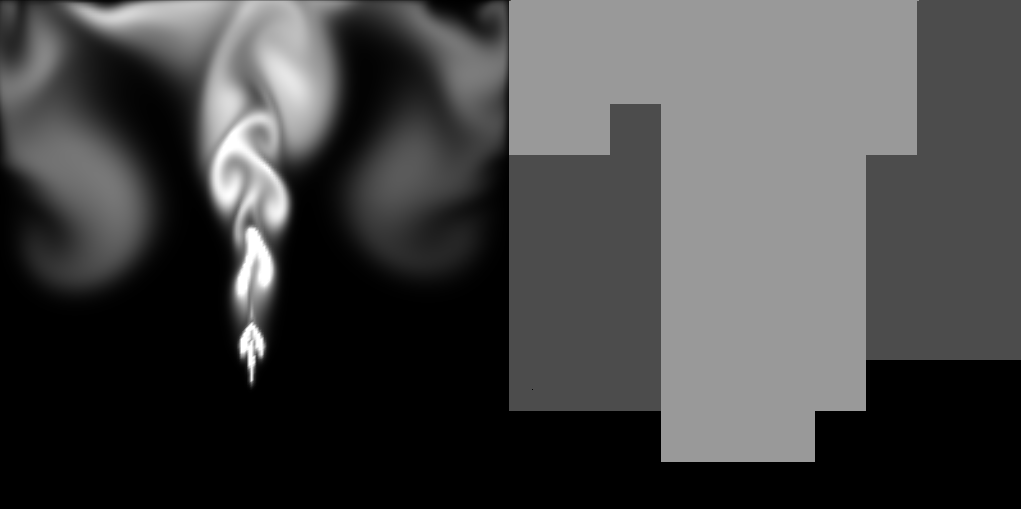
\includegraphics[scale=0.1]{img/logo.png} }

\subject{ Presentaci\'on Tesina 2017 } % \tiny{ }

\date{ \today} % \today will show
%current date.

\setbeamertemplate{navigation symbols}{}%remove navigation symbols 

%custom beaver footnote do what ever u want
\setbeamertemplate{footline} {%
\leavevmode
%
\hbox{%
\begin{beamercolorbox}[wd=.323\paperwidth,ht=2.25ex,dp=1ex,center]
    {author in head/foot}%
    \usebeamerfont{author in head/foot} Universidad Nacional de Rosario
\end{beamercolorbox}
%
\begin{beamercolorbox}[wd=.333\paperwidth,ht=2.25ex,dp=1ex,center]
    {title in head/foot}%
    \usebeamerfont{title in head/foot}\insertshorttitle
\end{beamercolorbox}
%
\begin{beamercolorbox}[wd=.3333\paperwidth,ht=2.25ex,dp=1ex,right]
    {date in head/foot}%
    \usebeamerfont{date in head/foot}\insertshortdate{}\hspace*{2em}
    \insertframenumber{} / \inserttotalframenumber\hspace*{1ex}
\end{beamercolorbox}
}%
\vskip0pt%
}

%\logo{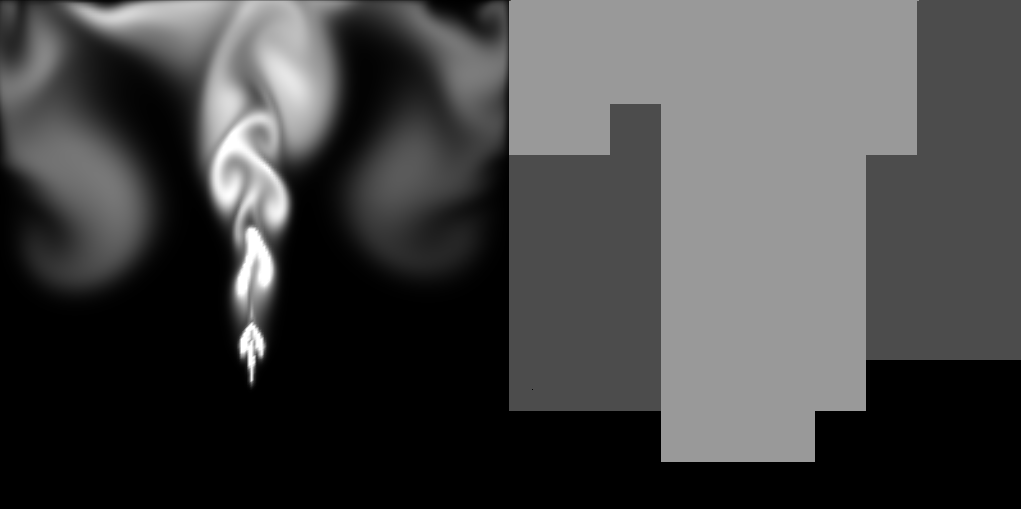
\includegraphics[scale=.04]{img/logo.png}}

\newcommand\codeHighlight[1]{\textcolor[rgb]{1,0,0}{\textbf{#1}}}

\newenvironment{rcases} {\left.
\begin{aligned}
    } {%
\end{aligned}
\right\rbrace}

\begin{document}
%
{ \setbeamertemplate{logo}{}
\begin{frame}
    \titlepage
    \vspace*{-25px}
    \begin{center}
        \large{ Presentaci\'on de Tesina }
    \end{center}

\end{frame}
}

%%%%%%%%%%%%%%%%%%%%%%%%%%%%%%%%%%%%%%%%%%%%%%%%%%%%%%%%%%%%%%%%%%%%%%%%%%%%%%%%
\begin{frame}
    \frametitle{Simulation}
    %more concrete simualtions, but a more abstract kind of problem
    \begin{itemize}
        \item
			A simulation is a program that immitates the behavior of a system over time
		\item
			It implements the abstract model describing the system
		\item
			\textbf{Usssually, it requires a big ammount of computing power }
    \end{itemize}
    	\begin{figure} 
	 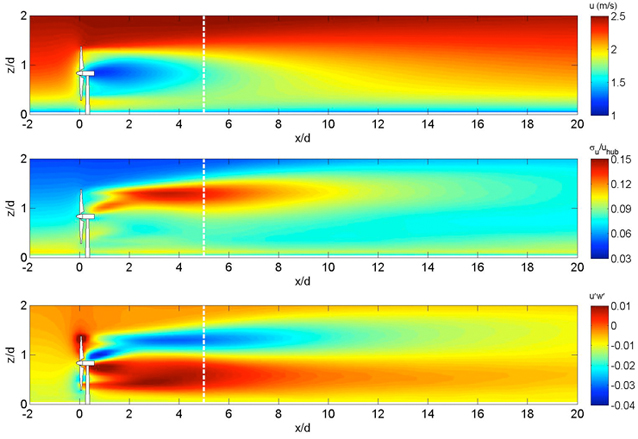
\includegraphics[scale=0.18]{img/wind_sim.jpg}
    \end{figure}
\end{frame}
%%%%%%%%%%%%%%%%%%%%%%%%%%%%%%%%%%%%%%%%%%%%%%%%%%%%%%%%%%%%%%%%%%%%%%%%%%%%%%%%

% End of slides
\end{document}



